\section{Definitions}

\subsection*{Graph}
    \addcontentsline{toc}{subsection}{Graph}

    Graph is a tuple $\left( V, E \right)$, where $V$ is the set of all nodes $v$, and $E$ is the set of edges $e_i = (v_j, v_k)$.

    Graphs can be undirected ($(v_j, v_k) \equiv (v_k, v_j)$) and directed, where presence of the edge $(v_j, v_k)$ does not imply that edge $(v_j, v_j)$ exists.
    Edges can also have weights which show some information about the tightness of connection of two nodes.
    In this case $e_i = (v_j, v_k, w_i)$.

    For instance, a road map of a country is an undirected weighted graph, where cities are nodes, roads are edges, and distances are weights.


\subsection*{Clique}
    \addcontentsline{toc}{subsection}{Clique}

    A graph clique is a subset of its nodes such that it is fully connected.
    So, n-clique is a set of $n$ nodes and $\frac{n \cdot (n - 1)}{2}$ edges~\cite{wiki_clique}.

    \begin{figure}[h]
        \centering
        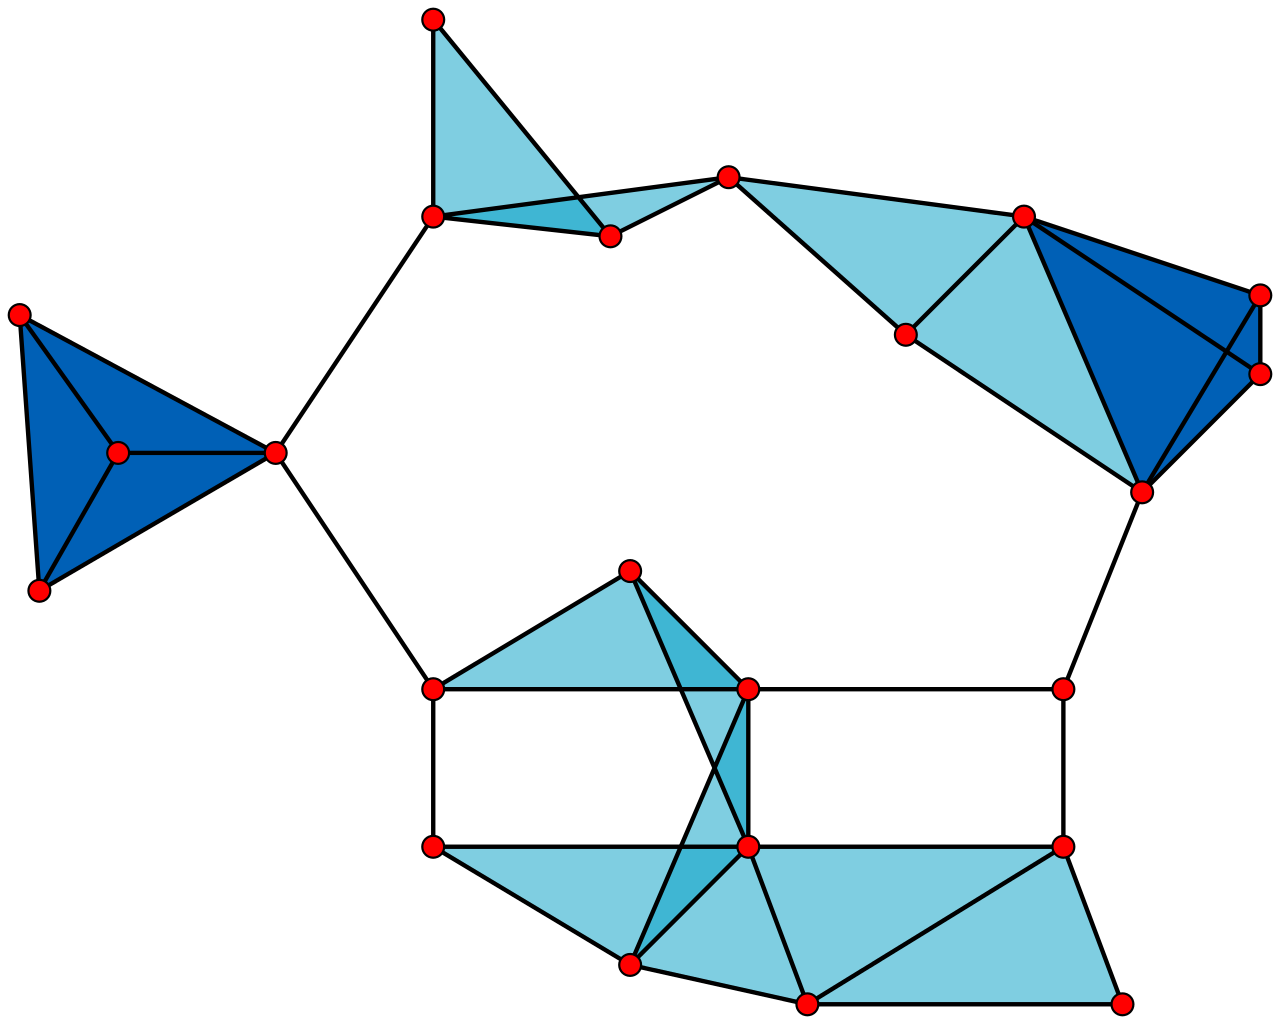
\includegraphics[width=0.4\textwidth]{clique.png}
        \caption{A graph with 23 1-vertex cliques (the vertices), 42 2-vertex cliques (the edges), 19 3-vertex cliques (light and dark blue triangles), and 2 4-vertex cliques (dark blue areas).}
    \end{figure}


\subsection*{Adjacency Matrix}
    \addcontentsline{toc}{subsection}{Adjacency Matrix}

    $\lvert V \rvert \times \lvert V \rvert$ adjacency matrix $A$ is defined as follows: $A_{i, j} = 1$ if there is an edge from $v_i$ to $v_j$.
    In our project we will consider undirected graphs with self-loops.
    This means that $\forall i, j\ A_{i, j} = A_{j, i}$ and $\forall i\ A_{i, i} = 1$.


\subsection*{Incidence Matrix}
    \addcontentsline{toc}{subsection}{Incidence Matrix}

    If we have an undirected graph $(V, E)$, its incidence matrix $\nabla$ of size $\lvert V \rvert \times \lvert E \rvert$ such that $A_{i, j} = 1$ if $i$-th vertex is a vertex of $j$-th edge.
    In directed case, we mark the initial vertex as -1, and the terminal as 1.

    \begin{multicols}{2}
        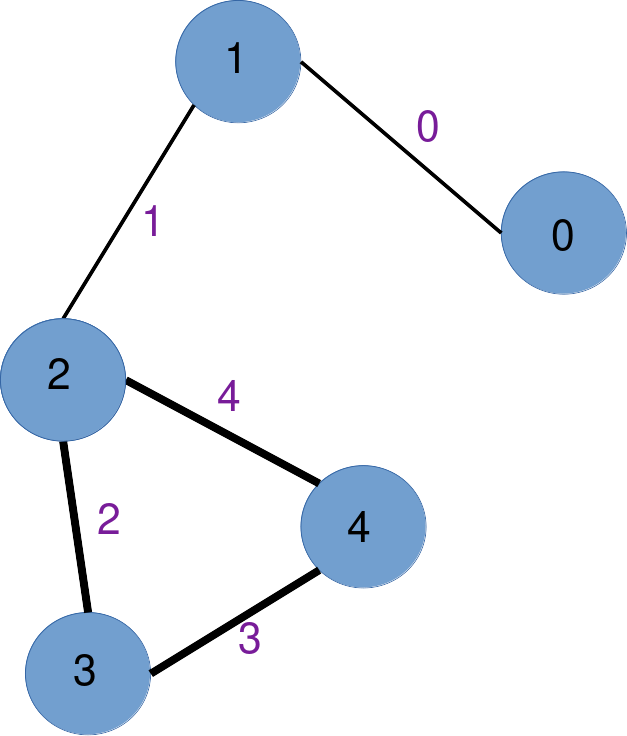
\includegraphics[width=0.3\textwidth]{incidence.png}

        The incidence matrix of the graph on the left would be as follows:

        \[
        \begin{bmatrix}
            1 & 0 & 0 & 0 & 0\\
            1 & 1 & 0 & 0 & 0\\
            0 & 1 & 1 & 0 & 1\\
            0 & 0 & 1 & 1 & 0\\
            0 & 0 & 0 & 1 & 1\\
        \end{bmatrix}
        \]

    \end{multicols}


\subsection*{Degree Matrix}
    \addcontentsline{toc}{subsection}{Degree Matrix}

    $\lvert V \rvert \times \lvert V \rvert$ diagonal degree matrix $D$ is defined as follows: $D_{i,i} = \Sigma_j A_{i, j}$ (that is, $D_{i, i} = in\_degree(v_i) + out\_degree(v_i)$)


\subsection*{Laplacian matrix}
    \addcontentsline{toc}{subsection}{Graph Laplacian}

    \textbf{Laplacian matrix} --- A matrix representation of a graph.
    Usually is calculated using the following formula~\cite{wiki_laplacian}:
    \begin{equation*}
        L_{i, j} = 
        \begin{cases}
            \deg(v_i) & \mbox{if}\ i = j \\
            -1 & \mbox{if}\ i \neq j\ \mbox{and}\ v_i \mbox{ is adjacent to } v_j \\
            0 & \mbox{otherwise},
    \end{cases}
    \end{equation*}

    However, other definitions also take place: $L = D - A$, where $D$ is a degree matrix and $A$ is an adjacency matrix.
    Another way to calculate a Laplacian is $L = \nabla\nabla^{T}$, where $\nabla$ is an incidence matrix.


\subsection*{Convolutional Graph Network}
    \addcontentsline{toc}{subsection}{Convolutional Graph Network}

    \textbf{CGN} \textit{(Convolutional Graph Network)} --- A type of GNN which generalizes the convolution operation to graphs.
    Often we encounter convolution while we work with grid-structured data like images, but here we use same idea (aggregate features of the neighbors) on nodes instead of pixels~\cite{9046288}.

    \begin{figure}[h]
        \begin{multicols}{2}
            \centering
            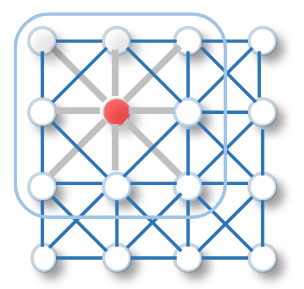
\includegraphics[width=0.25\textwidth]{conv.png}
            \caption{Convolution on image}
        
            \centering
            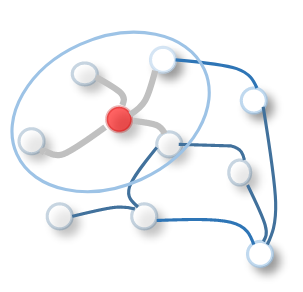
\includegraphics[width=0.25\textwidth]{CGN_conv.png}
            \caption{Convolution on graph}
        \end{multicols}
    \end{figure}

    Assume we have a graph of $N$ nodes, where each node has $F$ features.
    We can construct an $N \times F$ matrix called feature matrix.
    The first layer takes the feature matrix, and performs the following operation: $Z = D^{-\frac{1}{2}} A D^{-\frac{1}{2}} X W$, where: 
    \begin{itemize}
        \item $Z$ is resulting $N \times C$ signal
        \item $D$ is $N \times N$ degree matrix
        \item $A$ is $N \times N$ adjacency matrix with self-loops
        \item $X$ is $N \times F$ feature matrix (input signal)
        \item $W$ is $F \times C$ learnable weight matrix
    \end{itemize}

    Then the output $Z$ is directed into next layer, which does practically the same.
    There might be many convolutional layers, but usually models only have 2.

    The last (output) layer usually applies softmax function to each row resulting in a new matrix $S$.
    Then, in order to classify a node $v_i$ we simply take the index of maximum of $S_i$.
    

\subsection*{Graph Attention Network}
    \addcontentsline{toc}{subsection}{Graph Attention Network}

    \textbf{GAT} \textit{(Graph Attention Network)} --- A type of GNN which uses attention mechanism (also borrowed from `casual' neural networks) which allows us to work with inputs of variable sizes and to focus on the most important features~\cite{velickovic2018graph}.
    The attention mechanism is a function $a: \mathbb{R}^C \times \mathbb{R}^C \rightarrow \mathbb{R}$ which takes two feature vectors $X_i, X_j$ and returns a scalar representing how tight the connection between $v_i$ and $v_j$ is.

    We introduce an $N \times N$ matrix $e$ storing the attention between the nodes: $e_{i, j} = a\left( W \cdot X_i,\ W \cdot X_j \right)$.
    Now we have to be careful about choice of $i$ and $j$, since if we calculate the attention between all the nodes, we will completely drop structural information of the graph.
    One suggested solution is to use a neighborhood $\mathcal{N}_i$ of a vertex $v_i$ and then compute $e_{i, j}$ for all $j \in \mathcal{N}_i$.
    Existing model~\cite{velickovic2018graph} uses neighborhood of size 1 (that is, $v_i$ itself and all of its neighbors $v_j$ such that $\exists e = (v_i, v_j)$), and it seems to perform great.

    One might also want to normalize the coefficients.
    In order to do that, we can apply softmax function: $c_{i, j} = \text{softmax}_j (e_{i, j}) = \frac{\text{exp}(e_{i, j})}{\Sigma_k \text{exp}(e_{i, k})}$.
